\subsection{Storage of fields and index arrays}
\label{subsec:storage}

While the spinor fields are stored in even/odd order, the gauge
fields in lexicographial order.

In order to allow for continuous
memory access of the gauge fields (without being strided) in the
hopping matrix one can install a copy of the gauge field in correct
order. Ordered exactly in the order they are accessed in the hopping
matrix. The price for this trick is more memory requirement
and the need to copy the gauge field once. The time for copying is
negligible if it is done for instance once before an inversion of the
Dirac operator, during which the gauge fields stay constant. This
trick is switched on by the configure option {\ttfamily
  --enable-gaugecopy}.

Note that the additional memory needs might also affect the cash
coherency and moreover, your application might run out off memory.

\subsubsection{Space-time index arrays}

In general the fastest index is the z-direction, then the y-, x- and
time-direction. The local gauge field volume has size
{\ttfamily T*LX*LY*LZ=VOLUME}. 

The spinor fields have only size {\ttfamily (VOLUME)/2}. Thus
there are either only even or only odd sites stored. The two
index arrays called {\ttfamily lexic2eo} and {\ttfamily eo2lexic} map
from lexical to even/odd order and vice versa. {\ttfamily
  eo2lexic[ix]} returns the lexical index where {\ttfamily ix} is a
even/odd index and {\ttfamily lexic2eo[ix]} returns the even/odd index
where {\ttfamily ix} is now a lexical index. {\ttfamily lexic2eosub}
maps the lexical index to the even/odd index in a spinor field of half
size, thus either with only odd or with only even points.

This means that {\ttfamily lexic2eo} and {\ttfamily eo2lexic} return
values between {\ttfamily 0} and {\ttfamily VOLUME} in even/odd order
or in lexical oder, respectively. In case of even/odd order there are
first the even points and then the odd points. Since the spinor
fields have only length {\ttfamily (VOLUME)/2} we need to subtract
{\ttfamily (VOLUME)/2} in case of odd points, which is automatically
done by {\ttfamily lexic2eosub} taking values between {\ttfamily
0} and {\ttfamily VOLUME/2}. Therefore, by using {\ttfamily lexic2eosub}
the information on whether the point is even or odd is lost, but the
index can be used immediately in the actual spinor arrays due to its
correct range.

With the index array {\ttfamily g\_ipt[t][x][y][z]} one can map the
point $(t,x,y,z)$ to the lexical index. The indices of the next
neighbours of point with lexical index {\ttfamily ix} in forward and
backward direction $\mu$ you can get with
{\ttfamily g\_iup[ix][$\mu$]} and {\ttfamily g\_idn[ix][$\mu$]}
respectively.

In case the gauge fields are stored with even/odd order the even
fields are stored first. 

\subsection{Parallelisation}

The whole lattice can be parallelised in up to 4 space-time directions.
It is controled with the configure switches {\ttfamily --enable-mpi}
and {\ttfamily --with-mpidimension=1|2|3|4}. 

\subsubsection{One dimesional parallelisation}

In this situation only the time direction is parallelized. {\ttfamily
  T} is set to the local time extension. The global time extension is
given by {\ttfamily T*g\_nproc\_t}, where {\ttfamily g\_nproc\_t}
contains the number of processors in time direction. The local time
extension must be equal on each processor. Note that in the input file
the global time extension must be specified. 

In case the gauge fields are stored in lexical order the local gauge
fields are located first in memory with indices {\ttfamily 0 to
  T*LX*LY*LZ-1}, then come the right boundary fields ({\ttfamily t=T})
with indices {\ttfamily T*LX*LY*LZ} to {\ttfamily (T+1)*LX*LY*LZ-1}
and then the left boundary fields with index {\ttfamily
  (T+1)*LX*LY*LZ} to {\ttfamily (T+2)*LX*LY*LZ-1}. 

The amount needed for the boundary fields is defined to be {\ttfamily
  RAND}, such that {\ttfamily VOLUME+RAND=VOLUMEPLUSRAND=2*LX*LY*LZ}
is the total gauge field size and {\ttfamily (VOLUME+RAND)/2} the
total size of a (half) spinor field. 

In case of even/odd ordering for the gauge fields the storage in
memory is as follows: first come the even local gauge fields, then the
right even boundary fields, then the left even boundary fields, then
the odd local fields and then the odd boundary fields correspondingly.

The spinor fields are stored with the local fields first, then the
right and then the left boundary fields.  

Note that in the case of one dimensional parallelization the edges do
not need extra care since they are available in the boundary
automatically. 

\subsubsection{Two dimensional parallelisation}

When the two dimensional parallelization is used the time- and
x-direction are parallelized. Now {\ttfamily T} and {\ttfamily LX}
correspond to the local time- and x-extension of the lattice,
respectively. The global extensions are obtained by multiplying with
{\ttfamily g\_nproc\_t} and {\ttfamily g\_nproc\_x}. Again, in the
input file the global time- and x-extensions must be specified. 

In this case the storage of boundaries and the exchange procedures are
more complicated. The procdure is represented schematically in figure
\ref{fig:partition}). 

\begin{figure}[htbp]
\centering
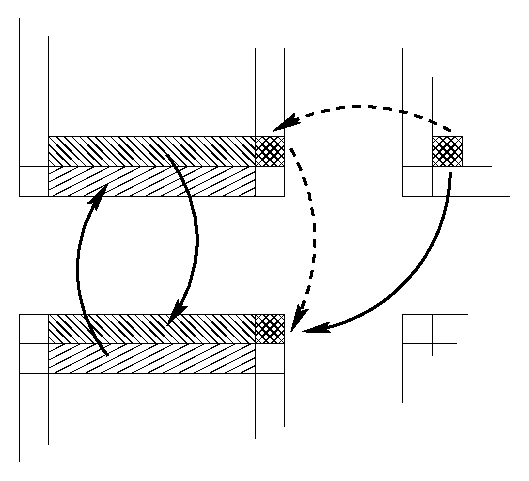
\includegraphics[width=0.65\linewidth]{partition}
\caption{Boundary exchange in a two dimensional parallel setup. One
  can see that the internal boundary is sended while the external one
  is received. The edges need a two step procedure.}
\label{fig:partition}
\end{figure}

In general the order for gauge and spinor fields in memory is as
follows: first the local fields, then the right t-boundary fields, then
the left t-boundary fields, then the right x-boundary fields, the left
x-boundary fields and finally the edges (see figure
\ref{fig:partition}. {\ttfamily RAND} is now defined to be {\ttfamily
  2*LY*LZ*(LX+T)} not including the edges, which are included only in
{\ttfamily VOLUMEPLUSRAND = LY*LZ*(T+2)*(LX+2)}. (Note that this means
{\ttfamily VOLUME+RAND} is not equal to {\ttfamily VOLUMEPLUSRAND} in
the two dimensional parallelization for historical reasons!)

\subsubsection{MPI setup}

The parallelization is setup using MPI. In particular, the number of
available processors is mapped to a cartesian grid using the
corresponding MPI functionality (see the MPI documentation for
details). Therefore in the input file only the number of processors in
x-direction must be specified (and only in the case of a two
dimensional parallelisation). The number of processors in
time-direction is computed automatically, which means that the
executable is independent of the number of processors used in the
actual run.

In the case of two dimensional parallelisation the internal boundary
in x-direction is not continous anymore, but strided. Therefore
{\ttfamily MPI\_Type\_vector} is used in order to avoid to copy the data
in a send buffer before sending it. Note that the external boundary is
still continuous.

The MPI setup is contained in the function {\ttfamily mpi\_init} that
must be called at the beginning of a main program just after the
parameters are read in, also in the serial case. In this function also
the various {\ttfamily MPI\_Datatype}s are constructed needed for the
exchange of the boundary fields.

The actual setup is controlled by several variables, which are all set
in {\ttfamily mpi\_init}:
\begin{itemize}
\item {\ttfamily g\_proc\_coords[]} containing the cartesian
  coordinates of the local processor in the MPI cartesian grid.
\item {\ttfamily g\_nproc} containing the global number of processors.
\item {\ttfamily g\_proc\_id} containing the processor id in the
  original MPI communicator {\ttfamily MPI\_COMM\_WORLD}.
\item {\ttfamily g\_nproc\_x, g\_nproc\_t} containing the number of
  processors in x- and time-direction.
\item {\ttfamily g\_cart\_id} containing the processor id in the MPI
  cartesian grid.
\item {\ttfamily g\_cart\_grid} containing the MPI communicator for
  the cartesian grid.
\item {\ttfamily g\_nb\_t\_dn}, {\ttfamily g\_nb\_t\_up}, {\ttfamily
    g\_nb\_x\_dn}, {\ttfamily g\_nb\_x\_up} containing the processor
  ids of the neighbouring processors in the corresponding direction in
  the cartesian grid.
\item {\ttfamily mpi\_time\_slices} containing a MPI communicator
  for a time-row in the cartesian grid. These communicators are needed
  for the computation of observables in the parallel setup.
\item {\ttfamily mpi\_time\_rank} containing the processor id in the
  time slice communicators.
\end{itemize}

\subsubsection{Exchange routines}

There are exchange routines available for the gauge fields ({\ttfamily
  xchange\_gauge}), for a (half) spinor field ({\ttfamily
  xchange\_spinor}) and for the derivatives ({\ttfamily xchange\_deri}),
respectively.

In the test directory there is a routine called {\ttfamily
  check\_xchange} which tests whether the exchange routines work correctly.


\begin{table}[t]
  \centering
  \begin{tabular*}{1.\textwidth}{@{\extracolsep{\fill}}ccc}
    \hline\hline
     & start address & size \\
    \hline\hline
    local volume & 0 & T*LX*LY*LZ \\
    \hline\hline
    t-Rand       & VOLUME & 2*LX*LY*LZ \\
    x-Rand       & ...+2*LX*LY*LZ & 2*T*LY*LZ\\
    y-Rand       & ...+2*T*LY*LZ & 2*T*LX*LZ \\
    z-Rand       & ...+2*T*LX*LZ & 2*T*LX*LY  \\
    \hline\hline
    xt-edge      & VOLUME+RAND  & 4*LY*LZ \\
    yx-edge      & ...+4*LY*LZ  & 4*T*LZ \\
    ty-edge      & ...+4*T*LZ   & 4*LX*LZ \\
    zx-edge      & ...+4*LX*LZ  & 4*T*LY\\
    tz-edge      & ...+4*T*LY   & 4*LX*LY\\
    zy-edge      & ...+4*LX*LY  & 4*T*LX\\
    \hline\hline
    t2-Rand      & VOLUMEPLUSRAND & 2*LX*LY*LZ \\
    x2-Rand      & ...+2*LX*LY*LZ & 2*T*LY*LZ \\
    y2-Rand      & ...+2*T*LY*LZ  & 2*T*LX*LZ \\
    z2-Rand      & ...+2*T*LX*LZ  & 2*T*LX*LY \\
    \hline\hline
    t2x-edge     & VOLUMEPLUSRAND+RAND & 4*LY*LZ \\
    x2t-edge     & ...+4*LY*LZ         & 4*LY*LZ \\
    x2y-edge     & ...+4*LY*LZ         & 4*T*LZ \\
    y2x-edge     & ...+4*T*LZ          & 4*T*LZ \\
    t2y-edge     & ...+4*T*LZ          & 4*LX*LZ \\
    y2t-edge     & ...+4*LX*LZ         & 4*LX*LZ \\
    t2z-edge     & ...+4*LX*LZ         & 4*LX*LY \\
    z2t-edge     & ...+4*LX*LY         & 4*LX*LY \\
    z2x-edge     & ...+4*LX*LY         & 4*T*LY \\
    x2z-edge     & ...+4*T*LY          & 4*T*LY \\
    z2y-edge     & ...+4*T*LY          & 4*T*LX \\
    y2z-edge     & ...+4*T*LX          & 4*T*LX \\
    \hline\hline
 \end{tabular*}
\end{table}

%%% Local Variables: 
%%% mode: latex
%%% TeX-master: "main"
%%% End: 
